\documentclass[11pt]{article}
%*******************************************************************
%--Packages
%*******************************************************************
\usepackage[final]{graphicx,epsfig}
\usepackage{subfigure}
\usepackage{subfigmat}
\usepackage{hyperref}
\newcommand{\noi}{\noindent}
\usepackage{listings}

\setlength{\parindent}{0pt}
\setlength{\parskip}{5pt plus 2pt minus 1 pt}
\topmargin  -5mm
\evensidemargin 8mm
\oddsidemargin  2mm
\textwidth  158mm
\textheight 230mm
%\renewcommand{\baselinestretch}{1.0}
\frenchspacing
\sloppy

\lstset{language=IDL,basicstyle=\footnotesize}

%%%%%%%%%%%%%%%%%%%%%%%%%%%%%%%%%%%%%%%%%%%%%%%%%%%%%%%%%%%%%%%%%%%%%%%

\begin{document}
\pagestyle{empty}

\begin{center}
  {\fontsize{14}{20}\bf 
    User-manual for COOLFluiD  \\
    (version 2017.10) \\[10pt]}
\end{center}

\begin{center}
  {Andrea Lani, \underline{lani@vki.ac.be} \\
    Von Karman Institute, Aeronautics \& Aerospace Dept.}
\end{center}

\section*{Introduction}

\noi
The COOLFluiD platform (\url{https://github.com/andrealani/COOLFluiD/wiki})
\cite{lani05, lani06, phd:lani, phd:quintino, phd:wuilbaut} is an object-oriented 
framework for high-performance computing (HPC) on unstructured grids and 
is the main in-house computational tool for CFD applications at the Von Karman Institute.
COOLFluiD consists of a set of plug-in libraries that 
can be linked at run-time to a kernel where the basic parallel
data structure and interface functionalities are defined.  
The platform is currently able to handle complex multi-physics simulations
with a wide range of spatial discretization algorithms
and time marching methods, both explicit and implicit.  
Linear systems arising from Newton linearizations of the space/time residual are efficiently solved 
in parallel with dedicated software packages that have been interfaced within COOLFluiD 
as plug-in libraries. Thanks to an extremely modular and scalable design, different 
functionalities (and corresponding library components) can be easily 
combined together to get more complex capabilities which will, in most cases, 
automatically work both serial and in parallel. Some of the available
features offered by the COOLFluiD software environment are:

\begin{itemize}
\item 
  {\bf multiple space discretizations:} Cell Centered Finite Volume (FV),  Residual Distribution (RD)
    Finite Element (FE), Spectral Finite Volume (SV), Spectral Finite Difference (SD), 
    Discontinuous Galerkin (DG);
  \item 
    {\bf multiple time integration schemes:} Runge Kutta, 1- and 3-point Backward Euler, Crank-Nicholson, Time limited schemes;
  \item
    {\bf multiple parallel linear system solvers:} PETsc, Trilinos, SAMG, Pardiso, jacobian free methods;
  \item
    {\bf parallel infrastructure:} parallel I/O capabilities and domain decomposition;
  \item 
    {\bf multiple physical models:} Ideal Magneto Hydro Dynamics (MHD), RANS ($k-\omega$, SST, BSL, Spalart-Allmaras models),
    Linear Elasticity, Heat Transfer, Compressible and Incompressible high-enthalpy flows in
    thermo-chemical nonequilibrium (TCNEQ) or in Local Thermodynamic Equilibrium (LTE)
    (with fixed or variable elemental fractions), Aeroacustics (LEE), LES;
  \item
    {\bf algorithms for loosely coupled multi-domain multi-physics simulations}: 
    different numerical methods applied to different models on full-non matching unstructured meshes 
    for Aeroelasticity, Aerothermoelasticity, Conjugate heat transfer, etc.
  \item
    {\bf ALE formulation for unsteady simulations on moving meshes}: high quality parallel mesh movement 
    and deformation algorithms.
  \end{itemize}
  The COOLFluiD platform has been {\bf designed to grow according to the needs} and has demonstrated its flexibility
  by incorporating progressively more and more complex algorithms and physical models. Some key strong points are:
  
\begin{itemize}
\item
  {\bf Flexible data-structure} that allows to implement 
  complex numerical methodologies and equations and get them 
  automatically working in parallel (all the described functionalities
  work in parallel!) to take full profit of computational power.
  The extreme flexibility is proved by the fact that is hard to find
  another software package, commercial or not, that can offer such 
  a variety of space discretization algorithms (each one with
  its own data-structure) working in parallel {\it within the same framework}.
\item
  {\bf Scalable design} that allows researchers to integrate new
  functionalities by fully reusing existing ones and take immediate 
  profit of others' work. As an example, physicists can work in 
  the Mutation library to refine the transport and thermodynamic 
  modeling and numericists can improve the numerical algorithms
  independently one from the other, or with extremely limited 
  interaction. At the end, the functionalities work
  both separately, as new independent framework components, and together.
\item
  {\bf Multi-physics} simulations can be customized at will, reusing the
  available components or incrementally implement new ones. 
\item
  {\bf State-of-the-art numerical algorithms} and {\bf extremely advanced
    physical modeling} for high-enthalpy flow properties (rigorously
  derived from kinetic theory or statistical and quantum mechanics)
  are combined together. 
\item
  Possibility of accurately simulating high-enthalpy flows {\bf from
    incompressible regime to hyper-velocity} (up to Mach 40 or more).
\end{itemize}

\section{Getting started}

Detailed installation instructions are available online at \url{https://github.com/andrealani/COOLFluiD/wiki/HOWTO}.
The following summarizes just the main steps for a standard installation and running of testcases.

\subsection{Installation instructions}

\begin{enumerate}
\item
  Download COOLFluiD sources: 
\begin{lstlisting}[breaklines]
svn co https://github.com/andrealani/COOLFluiD/trunk coolfluid
\end{lstlisting}
\item
  Running the script to install dependencies:
\begin{lstlisting}[breaklines]
cd coolfluid/tools/scripts
./install-coolfluid-deps.pl --tmp-dir=TDIR --install-dir=LDIR --install-mpi-dir=MDIR
\end{lstlisting}
  where \texttt{TDIR} is the full path to the directory where dependencies files will be unpacked,
  \texttt{LDIR} is the installation directory and \texttt{MDIR} is the directory where the 
  Message Passing Interface (MPI) libraries will be installed. PETSc and ParMetis libraries will be installed 
  inside the MPI directory. Different MPI installations can coexist: the user-defined \textit{coolfluid.conf} file,
  the \texttt{PATH} and \texttt{LD\_LIBRARY\_PATH} environmental variables will decide which actual installation to use.
\item
  Updating environmental variables to include the appropriate paths to the dependency libraries 
  in the \texttt{.bashrc}:
\begin{lstlisting}[breaklines]
  export PATH=LDIR/bin:MDIR/bin:$PATH
  export LD_LIBRARY_PATH=LDIR/lib:MDIR/lib:MDIR/petsc/lib:$LD_LIBRARY_PATH
\end{lstlisting}  
\item
  Setting up the file \textit{coolfluid.conf} with the appropriate \texttt{coolfluid\_dir},
  \texttt{basebuild\_dir}, \texttt{install\_dir}, paths to all dependencies (check example files in 
  \texttt{coolfluid/tools/conf}) and modules to download.
\item
  Checking out the selected modules with
\begin{lstlisting}[breaklines]
./prepare.pl --config-file=coolfluid.conf
\end{lstlisting}
\item
  Generating the build (make) files in \texttt{basebuild\_dir} in \textit{debug} (full debugging options, very slow), 
  \textit{optim} (some debug, some optimization, \textbf{recommended}) or \textit{release} (no debugging, full optimization) mode:
\begin{lstlisting}[breaklines]
./prepare.pl --config-file=coolfluid.conf --build=optim
\end{lstlisting}
\item 
  Compiling (typically on multiple cores, 4 in our example) and creating all COOLFluiD libraries:
\begin{lstlisting}[breaklines]
cd basebuild_dir ; make -j4 ; make install
\end{lstlisting}
\item 
  Setting the appropriate paths to the COOLFluiD libraries in the \texttt{.bashrc}:
\begin{lstlisting}[breaklines]
  export PATH=install_dir/bin:$PATH
  export LD_LIBRARY_PATH=install_dir/lib:$LD_LIBRARY_PATH
\end{lstlisting}  
\end{enumerate}

{\bf WATCH OUT:} {\it Steps 1 and 2 are only needed if dependency libraries are not installed in your system yet. Internal users at the VKI do not need those steps, since public installations are available. In particular, lammpi, openmpi and mpich2 are all supported at the VKI.
}  \\

{\bf WATCH OUT:} {\it Using "make install" in step 8 is not necessary if you choose to use soft links to the coolfluid-solver executable located in
  \texttt{basebuild\_dir/src/Solver} directory.  
}

\subsection{How to run a simulation (from inside a testcase folder)}

The command line to run COOLFluiD is: 

\begin{lstlisting}[breaklines]
mpirun -np N ./coolfluid-solver --scase ./myfile.CFcase
\end{lstlisting}
from inside the testcase directory. The parameter $N$ must be replaced by the number of 
processors. The format of the input file (called {\tt myfile.CFcase} in our example) is described here after.
For a serial run ($N$=1) the user can also use:

\begin{lstlisting}[breaklines]
./coolfluid-solver --scase ./myfile.CFcase
\end{lstlisting}

{\bf WATCH OUT:} {\it In order to be able to run successfully, a soft link to (or copy of) the {\tt coolfluid-solver} executable and file {\tt coolfluid-solver.xml} (providing useful info on the path to the COOLFluiD shared libraries) must be present in the working directory.}
 
\subsection{Configuration file description}

The format of the input file (with extension .CFcase) consists of lines in the form {\tt KEY} = {\tt VALUE}:
\vspace{-0.2cm}
\begin{lstlisting}[breaklines]
Simulator.OptionA = Value1               # use Value1 as value for OptionA
Simulator.Value1.OptionB = Value2        # use Value2 as value for OptionB
Simulator.Value1.Value2.OptionC = Value3 # use Value3 as value for OptionC
Simulator.Value1.Value2.OptionD = Value4 # use Value4 as value for OptionD
\end{lstlisting} 
where, in each line, the whole LHS is the keyword and the RHS is the value. The
latter, depending of the actual types defined in the code for each configurable parameter, can be:

\begin{itemize}
\item
  an alpha-numerical string
\item
  an integer
\item 
  a boolean (\texttt{true} or \texttt{false})
\item
  a floating point number
\item
  an arbitrarily complex analytical function
\item
  an array of all the previous.
\end{itemize}
The keyword is composed of literal strings separated by ".",
corresponding to different \textit{entities} (configurable
objects or parameters) defined inside the actual code. The
configuration is hierarchical and recursive from top to lowest
level. {\bf The order in which the options are declared in the file are
  irrelevant}. If needed, the value can be broken into different lines by using the continuation character (back slash) 
at the end of each line (note that the number of spaces at the end or
before the line is irrelevant):
\vspace{-0.2cm}
\begin{lstlisting}[breaklines]
Simulator.Example.arrays = 4 4 10 \
                           10 4 \
                           4 3
\end{lstlisting}
Comments start with "\#": they can occupy full lines or be placed at the end of the line.

\section{Environment options}

This section summarizes the main options available for setting up the kernel components of COOLFluiD (i.e. Environment and Framework libraries).

\begin{lstlisting}[breaklines]
CFEnv.ErrorOnUnusedConfig = true
\end{lstlisting}
If activated this option makes the simulation crash if there are spelling mistakes in the given options. This option must always be inactivated when using a mesh converter (e.g. Gambit2CFmesh, Gmsh2CFmesh, Tecplot2CFmesh).

\begin{lstlisting}[breaklines]
CFEnv.ExceptionDumps = true
CFEnv.ExceptionOutputs = true
\end{lstlisting}
If activated, those options will catch exceptions and show the error message. The simulation will crash only if the exception is not caught, but at least it will indicate what went wrong. It should be deactivated to reduce outputs in case things work.

\begin{lstlisting}[breaklines]
Simulator.Modules.Libs = libCFmeshFileReader libNavierStokes libFiniteVolume ...
\end{lstlisting}
List of the COOLFluiD dynamic libraries needed for the present simulation. In the following description, each section will indicate the required libraries whenever applicable.

\begin{lstlisting}[breaklines]
Simulator.Paths.WorkingDir = ./
Simulator.Paths.ResultsDir = ./RESULTS
\end{lstlisting}
Paths to the working directory and to the directory where output files (convergence history, Tecplot files, CFmesh files) should be written. 

\subsection{Interactive file}

Some parameters can be changed interactively during the simulation by editing a separate file
where the full option setting (key and value) has to be present.

\begin{lstlisting}[breaklines]
Simulator.SubSystem.InteractiveParamReader.FileName = ./out.inter
\end{lstlisting}
tells the path to the interactive file and
\begin{lstlisting}[breaklines]
Simulator.SubSystem.InteractiveParamReader.readRate = 10
\end{lstlisting}
specifies how often the file should be read by the solver in order to update the corresponding interactive parameters.\\
{\bf WATCH OUT:}  {\it In a parallel run, this rate must be defined with a safe margin (depending of the speed of the iterative process), 
  allowing the user to quickly edit, modify and close the file before the solver tries to read the file as well.}

\subsection{Stop Condition}

The simulation can be stopped by prescribing a maximum number of steps:

\begin{lstlisting}[breaklines]
Simulator.SubSystem.StopCondition = MaxNumberSteps
Simulator.SubSystem.MaxNumberSteps.nbSteps = 2
\end{lstlisting}
of by looking at the norm of the residual

\begin{lstlisting}[breaklines]
Simulator.SubSystem.StopCondition       = Norm
Simulator.SubSystem.Norm.valueNorm      = -3.0
\end{lstlisting}
A threshold of $<= -3.$ is reasonably good for most cases, if the temperature is used as variable to monitor (see MonitoredVarID below).

\begin{lstlisting}[breaklines]
Simulator.SubSystem.SubSystemStatus.TimeStep = 5.0
\end{lstlisting}
defines the time step in an unsteady simulation.

\section{Physical Model}

\subsection{Ideal MHD}

{\bf Required libs:~} libMHD.

\begin{lstlisting}[breaklines]
Simulator.SubSystem.Default.PhysicalModelType = MHD2DProjection (or MHD3DProjection)
\end{lstlisting}
defines a generic 2D (or 3D) ideal MHD model that uses hyperbolic divergence cleaning method as the $\nabla\cdot\vec{B}=0$ constraint satisfying technique.

\begin{lstlisting}[breaklines]
Simulator.SubSystem.Default.PhysicalModelType = MHD2D (or MHD3D)
\end{lstlisting}
defines a generic 2D (or 3D) ideal MHD model that uses Powell's source term method as the $\nabla\cdot\vec{B}=0$ constraint satisfying technique.

\begin{lstlisting}[breaklines]
Simulator.SubSystem.MHD3DProjection(or MHD3D or MHD2DProjection or MHD2D).ConvTerm.gamma = 1.666666667
\end{lstlisting}
defines the ratio of specific heats for the plasma which we take most of the time to be equal to 5/3.

\begin{lstlisting}[breaklines]
Simulator.SubSystem.MHD2DProjection(or MHD3DProjection).ConvTerm.refSpeed = 3.0
#Simulator.SubSystem.MHD2DProjection(or MHD3DProjection).ConvTerm.dissipCoeff = 3.0
#Simulator.SubSystem.MHD2DProjection(or MHD3DProjection).ConvTerm.correctionType = Mixed
\end{lstlisting}
defines a constant reference speed for the hyperbolic divergence cleaning method with hyperbolic Lagrange multiplier. The two commented out lines should be uncommented while using the mixed hyperbolic/parabolic Lagrange multiplier \cite{dedner02} which we never had to use so far. The constant reference speed is chosen to be equal to the freestream flow speed or the maximum speed in the initial conditions for unsteady simulations where there is no freestream flow in the setup of the testcase (see OrszagTang vortex, Smooth Alfv\'en Wave and Rotor testcases \cite{yalim11jcp}).  

\subsubsection{$\vec{B}_0+\vec{B}_1$ splitting model}

For solar wind/planetary magnetosphere interaction simulations, the planetary intrinsic magnetic field is modelled as a dipole ($\vec{B}_0$).

\begin{lstlisting}[breaklines]
Simulator.SubSystem.MHD3DProjection(or MHD2DProjection or MHD2D or MHD3D).ConvTerm.mX = 0.0
Simulator.SubSystem.MHD3DProjection(or MHD2DProjection or MHD2D or MHD3D).ConvTerm.mY = 0.0
Simulator.SubSystem.MHD3DProjection(or MHD3D).ConvTerm.mZ = -3000.0
\end{lstlisting}
define the magnetic dipole moment of the planetary magnetic field with the center of the dipole located at the origin.

\subsection{Thermochemical nonequilibrium}

{\bf Required libs:~} libNavierStokes, libNEQ.

\begin{lstlisting}[breaklines]
Simulator.SubSystem.Default.PhysicalModelType = NavierStokes2DNEQ
\end{lstlisting}
defines a generic 2D thermo-chemical nonequilibrium model.

\begin{lstlisting}[breaklines]
Simulator.SubSystem.NavierStokes2DNEQ.refValues = \
  1e-12 1e-6 1e-6 0.00002854 1e-6 0.00000866 1e-6 1e-6 \
  1e-6 1e-6 1e-6 11360. 1000. 195. 195.
\end{lstlisting}
provides values of the order of the free stream quantities for all stored variables (see {\tt .updateVar} below), one per equation. \\
{\bf WATCH OUT:} {\it None of those values can be zero, since they are actually used 
  as denominator in scaling for numerical finite difference while computing numerical jacobians. } 

\begin{lstlisting}[breaklines]
Simulator.SubSystem.NavierStokes2DNEQ.nbSpecies = 11
Simulator.SubSystem.NavierStokes2DNEQ.nbEulerEqs = 3
Simulator.SubSystem.NavierStokes2DNEQ.nbVibEnergyEqs = 1
\end{lstlisting}
specify the number of chemical species, the total number of equations excluding species continuity and vibrational/electronic equations 
(it must be $3$ for 2D cases, $4$ for 3D cases), the number of vibrational energy equations.

\subsubsection{Mutation 2.0}

{\bf Required libs:~} libMutation2OLD, libMutation2OLDI.

\begin{lstlisting}[breaklines]
Simulator.SubSystem.NavierStokes2DNEQ.PropertyLibrary = Mutation2OLD
\end{lstlisting}
specifies Mutation 2.0.0 (slower but stable version of Mutation 2.0) \cite{phd:magin, phd:panesi} as 
the physico-chemical library for computing thermodynamic, transport, chemical kinetics properties. This version of 
Mutation supports arbitrary chemical mixtures (neutral and ionized), chemical equilibrium models 
with fixed and variable elemental fractions, thermal and chemical nonequilibrium multi-temperature models, 
including full and reduced Collisional Radiative (CR) models for air \cite{panesi09}. 

\begin{lstlisting}[breaklines]
Simulator.SubSystem.NavierStokes2DNEQ.Mutation2OLD.mixtureName = air11
\end{lstlisting}
specifies the name of the mixture corresponding to a file {\tt air11.mix} defined inside \\
{\tt PATH\_TO\_MUTATION/Mutation2.0.0I/data/mixture}.

{\bf WATCH OUT:} {\it The mixture file specifies the order of the chemical species as they are used and stored by the flow solver.}  

\begin{lstlisting}[breaklines]
Simulator.SubSystem.NavierStokes2DNEQ.Mutation2OLD.reactionName = parkair93
\end{lstlisting}
specifies the name of the chemical reactions model corresponding to a file {\tt parkair93} defined inside 
{\tt PATH\_TO\_MUTATION/Mutation2.0.0I/data/chemistry/gasreact}.

\begin{lstlisting}[breaklines]
Simulator.SubSystem.NavierStokes2DNEQ.Mutation2OLD.transfName = air11
\end{lstlisting}
specifies the name of the energy transfer model corresponding to a file {\tt air11} defined inside 
{\tt PATH\_TO\_MUTATION/Mutation2.0.0I/data/chemistry/transfer}.

{\bf WATCH OUT:} {\it The detailed description of the format for Mutation data files is out of the scope of this tutorial. 
  The user is referred to the Mutation manual (contact {\tt magin@vki.ac.be}) instead.}  

\begin{lstlisting}[breaklines]
Simulator.SubSystem.NavierStokes2DNEQ.Mutation2OLD.TminFix = 100.
\end{lstlisting}
defines minimum temperature allowed inside Mutation routines.

\begin{lstlisting}[breaklines]
Simulator.SubSystem.NavierStokes2DNEQ.Mutation2OLD.dynViscAlgo = CG
Simulator.SubSystem.NavierStokes2DNEQ.Mutation2OLD.thermCondAlgo = Direct
\end{lstlisting}
specifies the transport algorithms to use for the computation of the dynamic viscosity and the thermal conductivity.
Those settings are the most stable and should not be changed.

\begin{lstlisting}[breaklines]
Simulator.SubSystem.NavierStokes2DNEQ.Mutation2OLD.includeElectronicEnergy = true
Simulator.SubSystem.NavierStokes2DNEQ.Mutation2OLD.electrEnergyID = 0
\end{lstlisting}
Those options should always be activated when running ionized cases and deactivated otherwise.

\begin{lstlisting}[breaklines]
Simulator.SubSystem.NavierStokes2DNEQ.Mutation2OLD.path = \
   /data1/andrea/COOLFLUID/plugins/Mutation2.0.0I/
\end{lstlisting}
provides the full path (no environmental variables are allowed here!) to the Mutation 2.0 installation.

\section{Output Format}

\begin{lstlisting}[breaklines]
Simulator.SubSystem.OutputFormat    = Tecplot CFmesh
\end{lstlisting}
defines list of requested output files (only {\tt Tecplot} and {\tt CFmesh} are supported for nonequilibrium flows).

\subsection{CFmesh writer}

{\bf Required libs:~} libCFmeshFileWriter
           
\begin{lstlisting}[breaklines]
Simulator.SubSystem.OutputFormat    = Tecplot CFmesh
\end{lstlisting}
defines list of requested output files (only {\tt Tecplot} and {\tt CFmesh} are supported for nonequilibrium flows).

\begin{lstlisting}[breaklines]
# in parallel runs, a file out-P0.CFmesh is written
Simulator.SubSystem.CFmesh.FileName = out.CFmesh  

# every how many iterations the file is saved  
Simulator.SubSystem.CFmesh.SaveRate = 1000

# append iteration number to the file name  	
Simulator.SubSystem.CFmesh.AppendIter = true
\end{lstlisting}
specifies the settings for the CFmesh file format (the internal format of COOLFluiD, including both mesh and solution).
Only one CFmesh file is written even in a parallel simulation. 

\subsection{Tecplot writer}

{\bf Required libs:~} libTecplotWriter.
        
\begin{lstlisting}[breaklines]
# in parallel runs, one file per processor out-P*.plt is written
Simulator.SubSystem.Tecplot.FileName       = out.plt

# output variables name (RhoivtTv correspond to [rho_i v T T_v])
Simulator.SubSystem.Tecplot.Data.outputVar = RhoivtTv

# write also density, total enthalpy, Mach number and pressure
Simulator.SubSystem.Tecplot.Data.printExtraValues = true  

# name of the boundary patch for which a file out-P*-surf.plt will be saved   
Simulator.SubSystem.Tecplot.Data.SurfaceTRS = Wall   

# every how many iterations the file is saved  
Simulator.SubSystem.Tecplot.SaveRate = 1000

# append iteration number to the file name
Simulator.SubSystem.Tecplot.AppendIter = false       
\end{lstlisting}
specifies the settings for the Tecplot file format. One file per processor will be written. 

\section{Mesh Creator}

\subsection{CFmesh reader}

{\bf Required libs:~} libCFmeshFileReader.

\begin{lstlisting}[breaklines]
Simulator.SubSystem.Default.listTRS = InnerFaces Wall Symmetry Inlet Outlet
\end{lstlisting}
specifies the list of all Topological Region Sets (TRS), i.e. the boundary patches as defined in the mesh file.
{\tt InnerFaces} dose not need to be included in the list.

\begin{lstlisting}[breaklines]
Simulator.SubSystem.MeshCreator = CFmeshFileReader
Simulator.SubSystem.CFmeshFileReader.Data.FileName = ./input.CFmesh
\end{lstlisting}
specify the reading from a file called {\tt Restart.CFmesh} in CFmesh format. 

\begin{lstlisting}[breaklines]
Simulator.SubSystem.CFmeshFileReader.Data.ScalingFactor = 1000. 
\end{lstlisting}
specifies a factor for which the input mesh must be {\it divided} (the name "Scaling" is misleading here). \\
{\bf WATCH OUT:} {\it the scaling factor must be used only when starting from scratch and not from a CFmesh file
  containing the solution.}
  
\begin{lstlisting}[breaklines]
Simulator.SubSystem.CFmeshFileReader.ParReadCFmesh.ParCFmeshFileReader.NbOverlapLayers = 2
\end{lstlisting}
This option is obsolete, but kept for compatibility with older versions of the code. It specifies the number 
of overlap layers in parallel computations. This value should be 2 for second-order calculations, 
but it is now automatically calculated.

\subsection{Converting from Gambit files}

{\bf Required libs:~} libGambit2CFmesh.

If the mesh file is not yet in CFmesh format and it's coming from the ANSYS Gambit mesh generator,
the following settings must e defined:  

\begin{lstlisting}[breaklines]
Simulator.SubSystem.CFmeshFileReader.convertFrom = Gambit2CFmesh
Simulator.SubSystem.CFmeshFileReader.Gambit2CFmesh.Discontinuous = true
Simulator.SubSystem.CFmeshFileReader.Gambit2CFmesh.SolutionOrder = P0
\end{lstlisting}
In this case the solver expects a file called {\tt input.neu} placed inside the working directory.
{\bf WATCH OUT:} {\it all Gambit settings must be commented out when restarting from a previous CFmesh solution 
  (see Restart option).}

\subsection{Converting from Gmsh files}

{\bf Required libs:~} libGmsh2CFmesh.

If the mesh file is not yet in CFmesh format and it's coming from the Gmsh mesh generator,
the following settings must e defined:  

\begin{lstlisting}[breaklines]
Simulator.SubSystem.CFmeshFileReader.convertFrom = Gmsh2CFmesh
Simulator.SubSystem.CFmeshFileReader.Gmsh2CFmesh.Discontinuous = true
Simulator.SubSystem.CFmeshFileReader.Gmsh2CFmesh.SolutionOrder = P0
\end{lstlisting}
In this case the solver expects {\tt input.msh} and {\tt input.SP} files placed inside the working directory
{\bf WATCH OUT:} {\it all Gmsh settings must be commented out when restarting from a previous CFmesh solution 
  (see Restart option).}

\subsubsection{Converting from THOR files}

{\bf Required libs:~} libTHOR2CFmesh.

If the mesh file is not yet in CFmesh format and it's coming from the THOR code mesh format,
the following settings must be defined:

\begin{lstlisting}[breaklines]
Simulator.SubSystem.CFmeshFileReader.THOR2CFmesh.Discontinuous = true
Simulator.SubSystem.CFmeshFileReader.THOR2CFmesh.SolutionOrder = P0
Simulator.SubSystem.CFmeshFileReader.convertFrom = THOR2CFmesh
\end{lstlisting}
In this case the solver expects a mesh file called {\tt input.thor} and a super patch file called {\tt input.SP} placed inside the working directory.\\
{\bf WATCH OUT:} {\it all THOR settings must be commented out when restarting from a previous CFmesh solution
  (see Restart option).}

\section{Convergence Method}

In the following {\tt <CMETHOD>} must be substituted with the concrete ConvergenceMethod name (e.g. BwdEuler, NewtonIterator, BDF2).

\subsection{Convergence file}

\begin{lstlisting}[breaklines]
  #the filename into which the convergence history is to be written
  Simulator.SubSystem.<CMETHOD.ConvergenceFile = ./convergence.plt
\end{lstlisting}

\subsection{CFL}
 
\subsubsection{Interactive CFL}

\begin{lstlisting}[breaklines]   
Simulator.SubSystem.<CMETHOD>.Data.CFL.ComputeCFL = Interactive
\end{lstlisting}
declares the CFL interactive and its value will be read from the interactive file ({\tt out.inter} in our example).
In this case the line
\begin{lstlisting}[breaklines]
Simulator.SubSystem.<CMETHOD>.Data.CFL.Interactive.CFL = 10.0
\end{lstlisting}
must be present and, if needed, modified in the interactive file.

\subsubsection{Function CFL}

\begin{lstlisting}[breaklines]   
Simulator.SubSystem.<CMETHOD>.Data.CFL.Value = 1.0
Simulator.SubSystem.<CMETHOD>.Data.CFL.ComputeCFL = Function
Simulator.SubSystem.<CMETHOD>.Data.CFL.Function.Def = \
  if(i<1000,1.0,if(i<2000.,1.01*cfl, min(1200.,1.05*cfl)))
\end{lstlisting}
In order to automatize the iterative process, a function specifying an arbitrarily complex CFL law can be provided.
The variable that can appear in this expression are: {\tt i} (iteration number), {\tt cfl} (previous CFL value), 
{\tt r} (current residual), {\tt ri} (initial residual), {\tt rl} (last residual), 
{\tt rmax} (maximum residual).

{\bf WATCH OUT:} {\it no spaces are allowed within the expression and the supported operators and mathematical functions
  are indicated in \cite{FParser}.}

\subsection{Backward Euler}

{\bf Required libs:~} libBackwardEuler libBackwardEulerMHD libNewtonMethod.

We consider here both the steady implicit time stepping case corresponding to a first-order accurate backward Euler integration and the unsteady implicit time stepping case corresponding to the second-order accurate Crank-Nicholson and BDF.

\begin{lstlisting}[breaklines]
Simulator.SubSystem.ConvergenceMethod = BwdEuler
#the filename into which the convergence history is to be written
Simulator.SubSystem.BwdEuler.ConvergenceFile = ./convergence.plt
\end{lstlisting}

\subsubsection{Backward Euler-MHD}

\begin{lstlisting}[breaklines]
Simulator.SubSystem.BwdEuler.UpdateSol = UpdateSolMHD
Simulator.SubSystem.BwdEuler.UpdateSolMHD.pressureCorrectionValue = 0.000000000001
\end{lstlisting}
define a correction value for negative pressure occurrences especially encountered during the solar wind/planetary magnetosphere simulations with sufficiently harsh initial conditions and planetary dipole field in the vicinity of the planet when started from an initial uniform solution. Thus, the simulation does not blow up due to the increase in the number of negative pressure occurrences and most of the time the negative pressure values are eliminated as the simulation continues.

\subsection{Newton Method}

{\bf Required libs:~} libNewtonMethod.

We consider here only the steady implicit time stepping case, corresponding to a first-order accurate 
Backward Euler integration.

\begin{lstlisting}[breaklines]
Simulator.SubSystem.ConvergenceMethod = NewtonIterator

# this value must be > 1 only for unsteady simulations
Simulator.SubSystem.NewtonIterator.Data.MaxSteps = 1
\end{lstlisting}
The CFL parameter which controls the stability of the calculation can be specified in two ways: 
interactively or with a user-defined function.

\begin{lstlisting}[breaklines]
Simulator.SubSystem.NewtonIterator.StdUpdateSol.Relaxation = 1.0
\end{lstlisting}
provides a relaxation parameter ($<= 1.0$): a single value for all equations or an array of values (with size equal to the number of equations).
This typically can be kept equal to 1.

\begin{lstlisting}[breaklines]
Simulator.SubSystem.NewtonIterator.Data.L2.MonitoredVarID = 13
\end{lstlisting}
indicates the ID of the variable to be monitored for convergence (see StopCondition). In chemically reacting flows, 
the ID corresponding to the temperature (total energy equation) is recommended.
\begin{lstlisting}[breaklines]
Simulator.SubSystem.NewtonIterator.Data.L2.ComputedVarID = 13
\end{lstlisting}
indicates the ID of the variable whose norm will be computed and written to screen. If this line is commented out, residuals 
for all variables will be computed.

\begin{lstlisting}[breaklines]
Simulator.SubSystem.NewtonIterator.Data.FilterState = Max

# flags (0 or 1) to tell which variables must be clipped
Simulator.SubSystem.NewtonIterator.Data.Max.maskIDs = \
 1 1 1 1 1 1 1 1 1 1 1 0 0 1 1

# real values to tell the minimum values to be imposed for each variable 
# only values given for flagged variables (maskID = 1) will be clipped
Simulator.SubSystem.NewtonIterator.Data.Max.minValues = \
 0. 0. 0. 0. 0. 0. 0. 0. 0. 0. 0. 0. 0. 0. 0.
\end{lstlisting}
provide some filtering of the solution values before the solution update.  

\subsection{BDF2}

\begin{lstlisting}[breaklines]
# this value must be > 1 only for unsteady simulations where it will represent the number of subiterations to be made at each timestep
Simulator.SubSystem.BDF2.Data.MaxSteps = 1
\end{lstlisting}

\begin{lstlisting}[breaklines]
Simulator.SubSystem.BDF2.Data.L2.MonitoredVarID = 8
\end{lstlisting}
indicates the ID of the variable to be monitored for convergence (see Stop condition). 
\begin{lstlisting}[breaklines]
Simulator.SubSystem.BDF2.Data.L2.ComputedVarID = 8 
\end{lstlisting}
indicates the ID of the variable whose norm will be computed and written to screen. If this line is commented out, residuals 
for all variables will be computed.

\begin{lstlisting}[breaklines]
Simulator.SubSystem.BDF2.Data.Norm = -3.
Simulator.SubSystem.BDF2.Data.PrintHistory = true
\end{lstlisting}

\section{Linear System Solver} \label{sec:LSS}

\subsection{PETSc}

{\bf Required libs:~} libPetsc.

We include here only the settings corresponding to the PETSC linear system solver library,
even though Trilinos is also interfaced within COOLFluiD.

\begin{lstlisting}[breaklines]
Simulator.SubSystem.LinearSystemSolver = PETSC
Simulator.SubSystem.LSSNames = NewtonIteratorLSS
Simulator.SubSystem.NewtonIteratorLSS.Data.PCType = PCASM
Simulator.SubSystem.NewtonIteratorLSS.Data.KSPType = KSPGMRES
Simulator.SubSystem.NewtonIteratorLSS.Data.MatOrderingType = MATORDERING_RCM
\end{lstlisting}
specify the basic settings for a GMRES solver combined with a parallel Additive Schwartz preconditioner.

\begin{lstlisting}[breaklines]
Simulator.SubSystem.NewtonIteratorLSS.Data.MaxIter = 1000
\end{lstlisting}
defines the maximum allowed number of GMRES iterations: should be typically kept $<= 1000$.

\begin{lstlisting}[breaklines]
Simulator.SubSystem.NewtonIteratorLSS.Data.RelativeTolerance = 1e-4
\end{lstlisting}
defines the relative tolerance for the GMRES solver: $1e-4$ or $1e-3$ are recommended values, since with higher values 
convergence can be very slow and requiring many more GMRES iterations per time step.

\section{Space Method: Finite Volume}

{\bf Required libs:~} libFiniteVolume

In order to restart from a previous CFmesh file (with saved solution), the following option must be set to true, 
otherwise must be commented out.
\begin{lstlisting}[breaklines]
Simulator.SubSystem.CellCenterFVM.Restart = true
\end{lstlisting}

\subsection{Initial Field}

The initial field conditions are typically prescribed on the full domain with a set of 
user-defined analytical functions depending on the position vector (x,y,z) \cite{FParser}, 
one for each of the update variables ({\tt RhoivtTv} in our current example). 

The following settings are always required:
\begin{lstlisting}[breaklines]
# "InitState" is the name of the object implementing an initial state 
Simulator.SubSystem.CellCenterFVM.InitComds = InitState

# "InField" is a user-defined alias that will be used to configure InitState
Simulator.SubSystem.CellCenterFVM.InitNames = InField

# from now on, only "InField" is used for the initialization settings
# "InnerFaces" is the boundary patch (TRS) on which InField is active
Simulator.SubSystem.CellCenterFVM.InField.applyTRS = InnerFaces
\end{lstlisting}

The following settings define the analytical functions.
\begin{lstlisting}[breaklines] 
# independent variables (use "x y z" in 3D)
Simulator.SubSystem.CellCenterFVM.InField.Vars = x y  

# arbitrarily complex function definitions (one per update variable, 15 in this case)
# no space allowed within a single function
# NOTE: this is just an illustrative example with no physical sense!
Simulator.SubSystem.CellCenterFVM.InField.Def = \
 0. 0. 0. if(sqrt(x^2+y^2)<1.,0.00002854,0.00002854/2.) \
 0. if(sqrt(x^2+y^2)<1.,0.00000866,0.00000866/2.) 0. 0. 0. 0. 0. 
 if(x<1.0,11360.,100.*(sqrt(x^2+y^2)-1.)) 0. 195. 195.
\end{lstlisting}

If analytical expressions are particularly complex, the user can use a more advance
2-step initializer. The previous example can be simplified as:

\begin{lstlisting}[breaklines]
# "InitStateAddVar" is used instead of "InitState"
Simulator.SubSystem.CellCenterFVM.InitComds = InitStateAddVar
Simulator.SubSystem.CellCenterFVM.InitNames = InField
Simulator.SubSystem.CellCenterFVM.InField.applyTRS = InnerFaces

Simulator.SubSystem.CellCenterFVM.InField.InitVars = x y
Simulator.SubSystem.CellCenterFVM.InField.InitDef = sqrt(x^2+y^2)

# here "rad" is a new user-defined variable that can be used 
# to simplify the final expressions 
Simulator.SubSystem.CellCenterFVM.InField.Vars = x y rad
Simulator.SubSystem.CellCenterFVM.InField.Def = \
 0. 0. 0. if(rad<1.,0.00002854,0.00002854/2.) \
 0. if(rad<1.,0.00000866,0.00000866/2.) 0. 0. 0. 0. 0. 
 if(x<1.0,11360.,100.*(rad-1.)) 0. 195. 195.
\end{lstlisting}

\subsection{Polynomial reconstruction}

The following options should be kept frozen:

\begin{lstlisting}[breaklines]
Simulator.SubSystem.CellCenterFVM.SetupCom = LeastSquareP1Setup
Simulator.SubSystem.CellCenterFVM.SetupNames = Setup1
Simulator.SubSystem.CellCenterFVM.Setup1.stencil = FaceVertexPlusGhost
Simulator.SubSystem.CellCenterFVM.UnSetupCom = LeastSquareP1UnSetup
Simulator.SubSystem.CellCenterFVM.UnSetupNames = UnSetup1
Simulator.SubSystem.CellCenterFVM.Data.PolyRec = LinearLS2D
Simulator.SubSystem.CellCenterFVM.Data.Limiter = Venktn2D
Simulator.SubSystem.CellCenterFVM.Data.Venktn2D.coeffEps = 1.0
Simulator.SubSystem.CellCenterFVM.Data.Venktn2D.useFullStencil = true
# set true the following for backward compatibility, but false should behave better
Simulator.SubSystem.CellCenterFVM.Data.Venktn2D.useNodalExtrapolationStencil = false
Simulator.SubSystem.CellCenterFVM.Data.Venktn2D.length = 1.0
\end{lstlisting}

The following factor determines if the simulation is of first, second or in-between order:

\begin{lstlisting}[breaklines]
# 0 <= gradientFactor <= 1, with  0. (first order), 1. (second order)
Simulator.SubSystem.CellCenterFVM.Data.LinearLS2D.gradientFactor = 0.
\end{lstlisting}
This is an interactive parameter that can be placed into the interactive file. Another interactive parameter,
important for second order computations, is 

\begin{lstlisting}[breaklines]
Simulator.SubSystem.CellCenterFVM.Data.LinearLS2D.limitRes = -4.0
\end{lstlisting}
This corresponds to the minimum residual at which the freezing of the flux limiter should be applied for flows exhibiting discontinuities 
or steep gradients (e.g., in temperature). In practice, {\tt limitRes} can be kept at  $-4$ till when the simulation reaches a limit cycle and then can be increased to
$8.$ in order to exit the cycle. This cure is not always effective and it often depends on the moment when {\tt limitRes} is increased.\\
{\bf WATCH OUT:} {\it Before restarting a simulation from a second order solution, if the limiter has not been explicitly saved in the CFmesh file 
  (see below), {\tt limitRes} has to be set back to $-4$.}

In order to save the limiter in second order calculations (when {\tt gradientFactor = 1.}), the following options must be added to the CFcase {\bf before} 
starting the computation:

\begin{lstlisting}[breaklines]
Simulator.SubSystem.CFmesh.Data.ExtraStateVarNames = limiter

# the following must be the total number of equations
Simulator.SubSystem.CFmesh.Data.ExtraStateVarStrides = 15
\end{lstlisting}

Finally, in order to restart from a file in which the limiter {\bf has been already saved}, 
the following line should be included in the CFcase file:

\begin{lstlisting}[breaklines]
Simulator.SubSystem.CFmeshFileReader.Data.ExtraStateVarNames = InitLimiter
\end{lstlisting}

\subsection{Finite Volume MHD}

{\bf Required libs:~} libFiniteVolume, libMHD, libFiniteVolumeMHD.

The following standard settings for the implicit FV solver should not be changed except the save rate which should be the same as the save rate of the Tecplot solution data file in order to be able to write the $\nabla\cdot\vec{B}$ error values correctly in the data file:

\begin{lstlisting}[breaklines]
Simulator.SubSystem.SpaceMethod = CellCenterFVM
Simulator.SubSystem.CellCenterFVM.ComputeRHS = NumJacobMHD
Simulator.SubSystem.CellCenterFVM.NumJacobMHD.SaveRate = 100
Simulator.SubSystem.CellCenterFVM.ComputeTimeRHS = StdTimeRhs (or BDF2TimeRhs when using BDF2)
Simulator.SubSystem.CellCenterFVM.BDF2TimeRhs.zeroDiagValue = 0 0 0 0 0 0 0 0 1
\end{lstlisting}
Moreover, with the last line, we make the time derivative of the last equation in the modified ideal MHD system due to the hyperbolic divergence cleaning vanish. Hence, we apply a pure Newton iteration on the last equation which reduced to the $\nabla\cdot\vec{B}=0$ constraint which is linear in $\vec{B}$ even after discretization. Thus, we assure convergence of the constraint upto machine accuracy even at each subiteration when using BDF2 \cite{yalim11jcp}.

\subsubsection{Interactive file}

For the present solver, the interactive parameters mainly utilized are the CFL number, diffusion reduction coefficient for the modified Rusanov scheme with tunable dissipation and the residual threshold value below which either the limiter is frozen or historical modification of limiter is applied as a remedy for convergence hampering for TVD schemes. The content of the interactive file in its most general form is given as follows:

\begin{lstlisting}[breaklines]
Simulator.SubSystem.BwdEuler(or BDF2).Data.CFL.Interactive.CFL = 1000.0
Simulator.SubSystem.CellCenterFVM.Data.LinearLS3D(or LinearLS2D).limitRes = -4.0
Simulator.SubSystem.CellCenterFVM.Data.LinearLS2D(or LinearLS3D).gradientFactor = 0.
Simulator.SubSystem.CellCenterFVM.Data.Centred.LaxFried.DiffCoeff = 0.3
Simulator.SubSystem.CellCenterFVM.Data.Centred.MHD3DProjectionConsLaxFriedTanaka(or MHD2DProjectionConsLaxFriedTanaka).DiffCoeff = 0.3
Simulator.SubSystem.CellCenterFVM.Data.Centred.MHD3DConsLaxFriedTanaka(or MHD2DConsLaxFriedTanaka).DiffCoeff = 0.3
\end{lstlisting}

\subsubsection{Convective flux schemes}

The user must choose one of the following (Rusanov scheme with tunable dissipation is recommended for most cases):

\begin{lstlisting}[breaklines]
Simulator.SubSystem.CellCenterFVM.Data.FluxSplitter = Centred
\end{lstlisting}
defines the option for Rusanov scheme. Specific cases that involve additional options were explained in detail earlier.

\begin{lstlisting}[breaklines]
Simulator.SubSystem.CellCenterFVM.Data.FluxSplitter = Roe
Simulator.SubSystem.CellCenterFVM.Data.Roe.Flux = MHD2DProjectionConsRoe (or MHD2DConsRoe or MHD3DProjectionConsRoe or MHD3DConsRoe)
\end{lstlisting}
define the option for Roe's scheme.

\paragraph{$\vec{B}_0+\vec{B}_1$ splitting method}

For solar wind/planetary magnetosphere interaction simulations, the planetary intrinsic magnetic field is modelled as a dipole ($\vec{B}_0$).

\begin{lstlisting}[breaklines]
Simulator.SubSystem.MHD3DProjection(or MHD2DProjection or MHD2D or MHD3D).ConvTerm.mX = 0.0
Simulator.SubSystem.MHD3DProjection(or MHD2DProjection or MHD2D or MHD3D).ConvTerm.mY = 0.0
Simulator.SubSystem.MHD3DProjection(or MHD3D).ConvTerm.mZ = -3000.0
\end{lstlisting}
define the magnetic dipole moment of the planetary magnetic field with the center of the dipole located at the origin.

\begin{lstlisting}[breaklines]
Simulator.SubSystem.CellCenterFVM.Data.Centred.Flux = MHD3DProjectionConsLaxFriedTanaka (or MHD3DConsLaxFriedTanaka or MHD2DConsLaxFriedTanaka or MHD2DProjectionConsLaxFriedTanaka)
Simulator.SubSystem.CellCenterFVM.Data.Centred.MHD3DProjectionConsLaxFriedTanaka(or MHD3DConsLaxFriedTanaka or MHD2DConsLaxFriedTanaka or MHD2DProjectionConsLaxFriedTanaka).NameFluxFunction = Powell99 (or Tanaka94)
\end{lstlisting}
define the necessary additional lines when using the Rusanov scheme together with the abovementioned type of problems. Note that in this type of problems Roe's scheme is not preferred as it was not observed to have the necessary robustness level. Therefore, we stick to the Rusanov scheme with tunable dissipation. Moreover, "Powell99" implementation made according to \cite{powell99} for only 3D problems is preferred over "Tanaka94" implementation made according to \cite{tanaka94} for both 2D and 3D problems as the latter implementation which involves matrix transformations is slower in comparison with the former. 

\subsubsection{Variable sets}

The following settings do not change for the present solver:

\begin{lstlisting}[breaklines]
Simulator.SubSystem.CellCenterFVM.Data.UpdateVar  = Cons
Simulator.SubSystem.CellCenterFVM.Data.SolutionVar = Cons
Simulator.SubSystem.CellCenterFVM.Data.LinearVar   = Cons
\end{lstlisting}

\subsubsection{Source terms}

\begin{lstlisting}[breaklines]
Simulator.SubSystem.CellCenterFVM.Data.hasSourceTerm = true
Simulator.SubSystem.CellCenterFVM.Data.SourceTerm = MHDConsACAST
\end{lstlisting}
should always be present in simulations involving hyperbolic divergence cleaning technique. 

\begin{lstlisting}[breaklines]
Simulator.SubSystem.CellCenterFVM.Data.hasSourceTerm = true
Simulator.SubSystem.CellCenterFVM.Data.SourceTerm = MHD2DPowellST (or MHD3DPowellST) 
\end{lstlisting}
should always be present in simulations involving Powell's source term technique.

\subsubsection{Boundary conditions}

Boundary condition fields will be applied also during initialization on the corresponding boundary TRS,
in such a way that {\it ghost states} (dummy cell centers that lie outside the computational domain) are set 
consistently before starting computing numerical fluxes. \\
The following example shows how to specify a full set of boundary conditions (three in this case, but 
real settings will obviously depend on the mesh in use).

\begin{lstlisting}[breaklines]
# list of the names of the objects defining each boundary condition
Simulator.SubSystem.CellCenterFVM.BcComds = \
      MirrorMHD3DProjectionTanakaPFixFVMCC \
      SuperInletFVMCC \
      SuperOutletMHD3DProjectionFVMCC

# list of aliases that the user must define for configuring each BC
Simulator.SubSystem.CellCenterFVM.BcNames = Wall Inlet Outlet
\end{lstlisting}

\begin{itemize}
\item
Ionosphere/magnetosphere boundary condition \cite{phd:yalim, yalim11jgr}

\begin{lstlisting}[breaklines]
# apply MirrorMHD3DProjectionTanakaPFixFVMCC to the SlipWall 
# (TRS name coming from the initial mesh file)
Simulator.SubSystem.CellCenterFVM.Wall.applyTRS = SlipWall

# imposed density and pressure 
Simulator.SubSystem.CellCenterFVM.Wall.rhoFixed = 1.0
Simulator.SubSystem.CellCenterFVM.Wall.pFixed = 8.0 (This value should be 8 times the freestream solar wind plasma pressure value which is equal to 1.0 in this example.) 
\end{lstlisting}
This boundary condition is based on \cite{powell99}.
\item
Superfast inlet boundary condition \cite{yalim08, phd:yalim, yalim11jcp, yalim11jgr}

\begin{lstlisting}[breaklines]
# apply SuperInletFVMCC to the SuperInlet TRS 
Simulator.SubSystem.CellCenterFVM.Inlet.applyTRS = SuperInlet
Simulator.SubSystem.CellCenterFVM.Inlet.Vars = x y z
Simulator.SubSystem.CellCenterFVM.Inlet.Def =  1.05100 \
                                        -3.99981 \
                                        0.283107 \
                                        -0.0381893 \
                                        0.403907 \
                                        0.399628 \
                                        -0.489089 \
                                        8.09741 \
                                        (0.0 in case of 9 equations)
\end{lstlisting}

\item
Superfast outlet boundary condition \cite{yalim08, phd:yalim, yalim11jcp, yalim11jgr}

\begin{lstlisting}[breaklines]
Simulator.SubSystem.CellCenterFVM.Outlet.applyTRS = SuperOutlet
Simulator.SubSystem.CellCenterFVM.Outlet.refPhi = 0.0
\end{lstlisting}
where the scalar potential function, $\phi$, value is kept constant in the ghost cells typically equal to 0 in all the testcases tried so far.
\end{itemize}

\subsection{Finite Volume NEQ (ATD)}

As far as the simulation of aerothermodynamics is concerned 
(see \cite{phd:lani, phd:panesi} for technical details), COOLFluiD offers: 
\begin{itemize}
\item 
  2D / axisymmetric / 3D FV solver for thermo-chemical equilibrium 
  (LTE with or without demixing effect) and NEQ 
  (different multi-temperature models) viscous flows 
  on unstructured hybrid grids with various schemes 
  (AUSM family, HUS, Roe, modified Steger-Warming, etc.).
\item 
  The same solver can also handle incompressible inductively coupled plasmas (ICP) in LTE 
  (extension to thermo-chemical NEQ is underway) where the Navier-Stokes equations 
  are weakly coupled with the electro-magnetic induction equations. 
\item
  COOLFluiD interfaces the Mutation F77 (version 2.0) and Mutation++ for the 
  accurate computation of thermodynamic, transport and chemical kinetics properties 
  in all temperature regimes, with different LTE and thermo-chemical NEQ models, 
  including pioneering collision-radiative models with $> 100$ chemical species \cite{munafo10}.
\item
  Simulations on neutral or ionized mixtures of argon, air, $CO_2$, nitrogen is available. 
\item 
  A new generation Residual Distribution solver for improving accuracy of 
  thermo-chemical NEQ flows simulations on unstructured simplex-element meshes 
  (with triangles or tetrahedra) is currently under development \cite{phd:lani}. 
\item
  Possibility of reusing all the available coupling algorithms to 
  get arbitrarily complex multi-physics steady or unsteady simulations 
  on deforming meshes \cite{phd:wuilbaut}.
\end{itemize}

{\bf Required libs:~} libFiniteVolume, libNavierStokes, libFiniteVolumeNavierStokes, libNEQ,  libFiniteVolumeNEQ. 

The following standard settings for the implicit Finite Volume solver should not be changed:

\begin{lstlisting}[breaklines]
Simulator.SubSystem.SpaceMethod = CellCenterFVM
Simulator.SubSystem.CellCenterFVM.ComputeRHS = NumJacobFast
Simulator.SubSystem.CellCenterFVM.NumJacobFast.FreezeDiffCoeff = true
Simulator.SubSystem.CellCenterFVM.ComputeTimeRHS = PseudoSteadyTimeRhs
\end{lstlisting}

\subsubsection{Convective flux schemes}

The user must choose one of the following convective flux schemes (AUSM+ is recommended for most cases):

The following work for both single- and multi-temperatures:
\begin{lstlisting}[breaklines]
# AUSM+ is the most stable and works for all equilibrium and NEQ models
Simulator.SubSystem.CellCenterFVM.Data.FluxSplitter = AUSMPlusMS2D
Simulator.SubSystem.CellCenterFVM.Data.AUSMPlusMS2D.choiceA12 = 5
\end{lstlisting}

\begin{lstlisting}[breaklines]
# AUSM+up flux works for all equilibrium and nonequilibrium models
# it includes some built-in preconditioning to handle low Mach flows
Simulator.SubSystem.CellCenterFVM.Data.FluxSplitter = AUSMPlusUpMS2D
Simulator.SubSystem.CellCenterFVM.Data.AUSMPlusUpMS2D.choiceA12 = 5
# the free stream Mach number must be specified
Simulator.SubSystem.CellCenterFVM.Data.AUSMPlusUpMS2D.machInf = 30.
\end{lstlisting}

\begin{lstlisting}[breaklines]
# HUS flux works for all NEQ models but is generally less stable and carbuncle prone
Simulator.SubSystem.CellCenterFVM.Data.FluxSplitter = HUSMS2D
Simulator.SubSystem.CellCenterFVM.Data.HUSMS2D.isNatural = true
\end{lstlisting}

The following scheme works only for two-temperatures and w/o ionization:
\begin{lstlisting}[breaklines]
# Roe scheme (Sanders' carbuncle fix) works only for neutral mixtures
# in thermo-chemical NEQ
Simulator.SubSystem.CellCenterFVM.Data.FluxSplitter = RoeTCNEQ2DSA 
Simulator.SubSystem.CellCenterFVM.Data.RoeTCNEQ2DSA.entropyFixID = 1  #2 or 3 
Simulator.SubSystem.NavierStokes2DNEQ.Mutation2OLD.noElectronicEnergy = true
\end{lstlisting}

\subsubsection{Variable sets for NEQ}

The following settings define some variable that are needed in different phases of the simulation.
In particular, the user should substitute {\tt <VARSET>} with {\tt Rhoivt} for single-temperature or {\tt RhoivtTv} for multi-temperature.

\begin{lstlisting}[breaklines]
# variables in which the solution is stored and updated 
# (use Rhoivt for thermal equilibrium)
Simulator.SubSystem.CellCenterFVM.Data.UpdateVar = <VARSET>

# variables in which the equations are formulated must ALWAYS be Cons
Simulator.SubSystem.CellCenterFVM.Data.SolutionVar = Cons

# variables in which the diffusive fluxes are computed 
# (use Rhoivt for thermal equilibrium)
Simulator.SubSystem.CellCenterFVM.Data.DiffusiveVar = <VARSET>

# diffusive flux must be NavierStokes for viscous computations
Simulator.SubSystem.CellCenterFVM.Data.DiffusiveFlux = NavierStokes
\end{lstlisting}

\subsubsection{2D and axisymmetric settings for NEQ}

\begin{lstlisting}[breaklines]
Simulator.SubSystem.CellCenterFVM.Data.isAxisymm = true
\end{lstlisting}
should always be present in 2D axisymmetric computations. \\

The following options must be activated only for axisymmetric calculations in thermo-chemical NEQ:

\begin{lstlisting}[breaklines]
# source terms for the axisymmetric case
Simulator.SubSystem.CellCenterFVM.Data.SourceTerm = \
  NavierStokes2DTCNEQAxiST Euler2DCTNEQST

# IDs corresponding to the velocity variables (momentum equations) 
Simulator.SubSystem.CellCenterFVM.Data.NavierStokes2DTCNEQAxiST.uvIDs = 11 12
\end{lstlisting}

The following options must be activated only for axisymmetric calculations in chemical NEQ (thermal equilibrium):

\begin{lstlisting}[breaklines]
# source terms for the axisymmetric case
Simulator.SubSystem.CellCenterFVM.Data.SourceTerm = \
  NavierStokes2DNEQAxiST Euler2DCNEQST

# IDs corresponding to the velocity variables (momentum equations) 
Simulator.SubSystem.CellCenterFVM.Data.NavierStokes2DNEQAxiST.uvIDs = 11 12
\end{lstlisting}

{\bf WATCH OUT:} {\it In 2D non-axisymmetric cases, only {\tt Euler2DCTNEQST} or {\tt Euler2DCNEQST} should be declared as source term.}

\subsubsection{Boundary Conditions}

Boundary conditions fields will be applied also during initialization on the corresponding boundary TRS,
in such a way that {\it ghost states} (dummy cell centers that lie outside the computational domain) are set 
consistently before starting computing numerical fluxes. \\
The following example shows how to specify a full set of boundary conditions (four in this case, but 
real settings will obviously depend on the mesh in use).

\begin{lstlisting}[breaklines]
# list of the names of the objects defining each boundary condition
Simulator.SubSystem.CellCenterFVM.BcComds = \
    NoSlipWallIsothermalNSrvtMultiFVMCC \
    MirrorVelocityFVMCC \
    SuperInletFVMCC \
    SuperOutletFVMCC

# list of aliases that the use must define for configuring each BC
Simulator.SubSystem.CellCenterFVM.BcNames = NSWall Mirror SInlet SOutlet
\end{lstlisting}

\paragraph{Noslip wall (isothermal, adiabatic or with radiative equilibrium)}

\begin{lstlisting}[breaklines]
# apply NoSlipWallIsothermalNSrvtMultiFVMCC to the Wall
# (TRS name coming from the initial mesh file)
Simulator.SubSystem.CellCenterFVM.NSWall.applyTRS = Wall

# if an adiabatic condition is needed set this flag to true
Simulator.SubSystem.CellCenterFVM.NSWall.Adiabatic = false

# imposed wall temperature
Simulator.SubSystem.CellCenterFVM.NSWall.TWall = 615.0

In order to impose a radiative equilibrium condition, additional options are needed:
\begin{lstlisting}[breaklines]
Simulator.SubSystem.CellCenterFVM.NSWall.RadEquilibrium = true

# emissivity
Simulator.SubSystem.CellCenterFVM.NSWall.Emissivity = 0.9

# maximum allowable change in temperature between two consecutive time step
Simulator.SubSystem.CellCenterFVM.NSWall.MaxRadEqDTwall = 100.

# temperature of the distant body (typically 0 or free stream value)
Simulator.SubSystem.CellCenterFVM.NSWall.DistantBodyTemp = 0.
\end{lstlisting}

A super-catalytic wall condition, imposing LTE at the wall, can be imposed by replacing 
the BC object name {\tt NoSlipWallIsothermalNSrvtMultiFVMCC} with 
{\tt NoSlipWallIsothermalNSrvtLTEMultiFVMCC}. 

\paragraph{Symmetry plane or slip wall}

\begin{lstlisting}[breaklines]
# apply MirrorVelocityFVMCC to the Symmetry TRS 
Simulator.SubSystem.CellCenterFVM.Mirror.applyTRS = Symmetry

# IDs corresponding to the velocity components 
# (they dependent on the chemical model in use)
Simulator.SubSystem.CellCenterFVM.Mirror.VelocityIDs = 11 12

# array of flags where "1" correspond to variables for which 
# a zero gradient has to be imposed
Simulator.SubSystem.CellCenterFVM.Mirror.ZeroGradientFlags = \
  1 1 1 1 1 1 1 1 1 1 1 0 0 1 1
\end{lstlisting}

\paragraph{Super inlet}

\begin{lstlisting}[breaklines]
# apply SuperInletFVMCC to the Inlet TRS
Simulator.SubSystem.CellCenterFVM.SInlet.applyTRS = Inlet

# analytical functions can be defined here as for InitState 
# (2-step option is not available though)
Simulator.SubSystem.CellCenterFVM.SInlet.Vars = x y
Simulator.SubSystem.CellCenterFVM.SInlet.Def = \
 0. 0. 0. 0.00002854 0. 0.00000866 0. 0. 0. 0. 0. 11360. 0. 195. 195.
\end{lstlisting}
specify the settings for a supersonic inlet (all RhoivtTv variables have to be prescribed).
Additional interactive parameters (to be put in the interactive file) can be used 
for running stiff cases (typically 3D), for which, for instance, it may be impossible 
to start with the full velocity:

\begin{lstlisting}[breaklines]
# the following settings tell the solver to multiply the variable with 
# ID = 11 (x-velocity) by a factor (must <= 1.0)
Simulator.SubSystem.CellCenterFVM.SInlet.InteractiveVarIDs = 11
Simulator.SubSystem.CellCenterFVM.SInlet.InteractiveFactor = 1.0
\end{lstlisting}

\paragraph{Super outlet}

\begin{lstlisting}[breaklines]
Simulator.SubSystem.CellCenterFVM.SOutlet.applyTRS = Outlet

# array of flags where "1" correspond to variables for which 
# a zero gradient has to be imposed
Simulator.SubSystem.CellCenterFVM.SOutlet.ZeroGradientFlags = \
  1 1 1 1 1 1 1 1 1 1 1 1 1 1 1
\end{lstlisting}

\subsubsection{Nodal Extrapolation}

Since flow solution is computed in the cell centers, nodal values must be extrapolated from cell centers 
to the mesh vertices for visualization purposes or for computing viscous gradients. This is accomplished by 
{\tt NodalExtrapolation} objects. In viscous NEQ cases, where a slip condition and, possibly, a temperature 
are imposed at the wall, the following settings must be added in order to strongly impose the desired values.

\begin{lstlisting}[breaklines]
# this specifies the name of the nodal extrapolator object
Simulator.SubSystem.CellCenterFVM.Data.NodalExtrapolation = DistanceBasedGMoveRhoivt

# the name(s) of the boundary TRS(s) on which imposing values strongly 
Simulator.SubSystem.CellCenterFVM.Data.DistanceBasedGMoveRhoivt.TRSName = Wall

# IDs of the variables to be imposed strongly on the boundaries listed in TRSName
Simulator.SubSystem.CellCenterFVM.Data.DistanceBasedGMoveRhoivt.ValuesIdx = \
  11 12 13 14

# values of the selected variables to be imposed strongly
Simulator.SubSystem.CellCenterFVM.Data.DistanceBasedGMoveRhoivt.Values = \
  0. 0. 615. 615.

# list determines the priority of one TRS (and BC) over another in corner nodes
Simulator.SubSystem.CellCenterFVM.Data.DistanceBasedGMoveRhoivt.TrsPriorityList = \
   Wall Symmetry Inlet Outlet
\end{lstlisting}

{\bf WATCH OUT:~} {\it Nodal extrapolation settings must be consistent with the boundary conditions (same velocity IDs, same temperature at the wall, etc.).}

\paragraph{Radiative equilibrium case}

When radiative equilibrium is imposed at the wall, besides specifying appropriate boundary condition settings (see above),
the nodal extrapolation must also be adapted consistently, as follows.

\begin{lstlisting}[breaklines]
# only velocity IDs and values must be prescribed at the wall nodes, since 
# temperature will be computed on-the-fly by an iterative procedure  
Simulator.SubSystem.CellCenterFVM.Data.DistanceBasedGMoveRhoivt.ValuesIdx = 11 12 
Simulator.SubSystem.CellCenterFVM.Data.DistanceBasedGMoveRhoivt.Values = 0. 0.

# this flag must be activated
Simulator.SubSystem.CellCenterFVM.Data.DistanceBasedGMoveRhoivt.RadEquilibrium = true
\end{lstlisting}

\paragraph{Super-catalytic case (LTE at the wall)}

A super-catalytic BC requires setting {\tt DistanceBasedGMoveRhoivtLTE} instead of  
{\tt DistanceBasedGMoveRhoivt}.

\subsubsection{Post-processing: radiation coupling and surface quantities computation}

We declare two post-processing numerical commands.

\begin{lstlisting}[breaklines]
# name of the post-processing objects
Simulator.SubSystem.DataPostProcessing = DataProcessing DataProcessing

# user-defined configuration names for the post-processing object 
Simulator.SubSystem.DataPostProcessingNames = DataProcessing2 DataProcessing3
\end{lstlisting}

\paragraph{Radiation coupling}

{\bf Required libs:~} libparade, libradiation, libParadeI, libRadiativeTransfer.

The following options control the postprocessing:

\begin{lstlisting}[breaklines]
# how often the post-processing is applied (this is an interactive option, 
# it can go to the interactive file)
Simulator.SubSystem.DataProcessing2.ProcessRate = 100

# flag telling if to skip the coupling for the first iteration (advised)
Simulator.SubSystem.DataProcessing2.SkipFirstIteration = true
\end{lstlisting}

The following options allow for solving the radiation transport on the stagnation line (works only in serial mode) 
using PARADE or to solve optically thin in the whole domain.

\begin{lstlisting}[breaklines]
# name of the command object implementing the radiation coupling
# Slab1DFVMCC corresponds to 1D infinite tangent slab method
Simulator.SubSystem.DataProcessing2.Comds = Slab1DFVMCC

# user-defined configuration name for "Slab1DFVMCC"
Simulator.SubSystem.DataProcessing2.Names = Radiation1D

# wall TRS boundary required by the algorithm 
Simulator.SubSystem.DataProcessing2.Radiation1D.applyTRS = Wall

# if this option is present, providing the x,y coordinates of the stagnation point,
# the RTE will be solved ONLY on the stagnation line
# this setting should be commented out in case all mesh lines are needed (not supported)
Simulator.SubSystem.DataProcessing2.Radiation1D.StagnationPoint = 0. 0.

# radiation library (only Parade is available at the moment)
Simulator.SubSystem.DataProcessing2.Radiation1D.RadiationLibrary = Parade

# flag telling if the flow is emission dominated (optically thin assumption) 
Simulator.SubSystem.DataProcessing2.Radiation1D.Parade.EmisDom = true

# temperature to impose on the wall boundary 
Simulator.SubSystem.DataProcessing2.Radiation1D.Parade.Tb1 = 615.0

# free stream temperature to impose on the inlet boundary 
Simulator.SubSystem.DataProcessing2.Radiation1D.Parade.Tb2 = 195.0

# under-relaxation factor (must be <= 1)
Simulator.SubSystem.DataProcessing2.Radiation1D.Parade.UndRel = 1.0
\end{lstlisting}

The following options allow for solving the radiation transport with the \textbf{Monte-Carlo} algorithm 
and to couple back the computed $\nabla \cdot {\bf q}_{rad}$ to the flow energy conservation equation. 

\begin{lstlisting}[breaklines]
# name of the command object implementing the radiation transport via Monte-Carlo
Simulator.SubSystem.DataProcessing2.Comds = RadiativeTransferMonteCarloFVMCC

# user-defined configuration name for "RadiativeTransferMonteCarloFVMCC"
Simulator.SubSystem.DataProcessing2.Names = RT

# Name of the topological region where to apply the algorithm
Simulator.SubSystem.DataProcessing2.RT.applyTRS = InnerFaces

# Names of the topological regions corresponding to solid walls
Simulator.SubSystem.DataProcessing2.RT.wallTrsNames = Wall1 Wall2

# Names of the topological regions corresponding to symmetry planes
Simulator.SubSystem.DataProcessing2.RT.symmetryTrsNames = Symmetry

# Names of the topological regions corresponding to other boundaries
Simulator.SubSystem.DataProcessing2.RT.boundaryTrsNames = Inlet Outlet

# User-defined number of rays (photons) shot by each computational cell 
Simulator.SubSystem.DataProcessing2.RT.numberOfRays = 20

# Maximum number of visited cell during ray tracing
Simulator.SubSystem.DataProcessing2.RT.MaxNbVisitedCells = 200

# Number of wavelengths to be considered to obtain a reduced spectra 
Simulator.SubSystem.DataProcessing2.RT.ReducedSpectralSize = 500

# Wall emissivity 
Simulator.SubSystem.DataProcessing2.RT.WallEmissivity = 0.

# Wall absorption coefficient 
Simulator.SubSystem.DataProcessing2.RT.WallAbsorption = 0.644

# ID of the temperature in the state vector 
# (typically = number of species + spatial dimension)
Simulator.SubSystem.DataProcessing2.RT.TemperatureID = 13

# Free stream temperature (if>0, it will impose q_rad=0 for the cell where active)
#Simulator.SubSystem.DataProcessing2.RT.FreeStreamTemperature = 640.

# Flag to tell to use the Planck function at the wall 
# (alternative to specifying WallEmissivity)
#Simulator.SubSystem.DataProcessing2.RT.PlanckFunction = true
\end{lstlisting}

In axisymmetric cases, the following must be specified:
 
\begin{lstlisting}[breaklines]
# Specify if to use the axisymmetric ray tracing
Simulator.SubSystem.DataProcessing2.RT.Axi = true

# Specify the number of cells in the streamwise direction
Simulator.SubSystem.DataProcessing2.RT.nCx = 80

# Specify the number of cells normal to the wall
Simulator.SubSystem.DataProcessing2.RT.nCy = 150
\end{lstlisting}

PARADE settings to be used in combination with Monte-Carlo:

\begin{lstlisting}[breaklines]
# radiation library (only Parade is available at the moment)
Simulator.SubSystem.DataProcessing2.RT.RadiationLibrary = Parade

# flag telling if the flow is emission dominated (optically thin assumption) 
Simulator.SubSystem.DataProcessing2.RT.Parade.EmisDom = false

# Minumum wavelength (must be consistent with "wavlo" declared in parade.con) 
Simulator.SubSystem.DataProcessing2.RT.Parade.WavelengthMin = 2000.

# Maximum wavelength (must be consistent with "wavhi" declared in parade.con) 
Simulator.SubSystem.DataProcessing2.RT.Parade.WavelengthMax = 40000.

# number of wavelengths for which radiative properties are computed at a time
# if < "npoints" declared in parade.con, Monte-Carlo will compute radiative properties
# for this number of wavelengths at once 
Simulator.SubSystem.DataProcessing2.RT.Parade.WavelengthStride = 10000

# Path where PARADE is installed with all data files
Simulator.SubSystem.DataProcessing2.RT.Parade.path = /home/myuser/PARADEv3.1/parade31

# when set to 1, this allows for restarting from previously computed radiative properties
# as long as the number of processors remains the same as in the previous run 
Simulator.SubSystem.DataProcessing1.RT.Parade.ReuseProperties = 0
\end{lstlisting}

The flow radiation cupoling is controlled by one interactive parameter (can be changed interactively inside the .inter file)

\begin{lstlisting}[breaklines]
# RadRelaxationFactor = 0       uncoupled case
# 0 < RadRelaxationFactor <= 1  coupled case, this is an under-relaxation factor    
Simulator.SubSystem.CellCenterFVM.Data.Euler2DCTNEQST.RadRelaxationFactor = 1.0
\end{lstlisting}

{\bf WATCH OUT:~} {\it In order to run the flow-radiation coupling the executable {\tt parade} together 
  with all required PARADE input files (parade.con) must be present in the working directory.}

\subsection{Surface quantities}

{\bf Required libs:~} libAeroCoefFVM, libAeroCoefFVMNEQ.

Surface quantities such as surface pressure, temperature, heat flux and skin friction
can be computed and saved to {\bf one single Tecplot file} with the following settings.

\begin{lstlisting}[breaklines]
# how often the post-processing is applied (this is an interactive option, 
# it can go to the interactive file)
Simulator.SubSystem.DataProcessing3.ProcessRate = 10

# name of the command object implementing the post-processing
Simulator.SubSystem.DataProcessing3.Comds = NavierStokesSkinFrictionHeatFluxCCNEQ

# user-defined configuration name for "NavierStokesSkinFrictionHeatFluxCCNEQ"
Simulator.SubSystem.DataProcessing3.Names = SkinFriction

# boundary TRS on which applying the post-process
Simulator.SubSystem.DataProcessing3.SkinFriction.applyTRS = Wall

# output Tecplot data file on which surface quantities will be written
Simulator.SubSystem.DataProcessing3.SkinFriction.OutputFileWall = walldata.plt

# ALL the following free stream values and update variable IDs MUST be specified
Simulator.SubSystem.DataProcessing3.SkinFriction.rhoInf = 0.0000372 # density
Simulator.SubSystem.DataProcessing3.SkinFriction.pInf = 2.1         # pressure
Simulator.SubSystem.DataProcessing3.SkinFriction.uInf = 11360.      # x-velocity
Simulator.SubSystem.DataProcessing3.SkinFriction.TInf = 195.        # temperature
Simulator.SubSystem.DataProcessing3.SkinFriction.UID = 11           # x-velocity ID
Simulator.SubSystem.DataProcessing3.SkinFriction.VID = 12           # y-velocity ID
Simulator.SubSystem.DataProcessing3.SkinFriction.TID = 13           # temperature ID
\end{lstlisting}

\section{Mesh Fitting Algorithms}

{\bf Required libs:~} libMeshTools, libMeshToolsFVM.

The COOLFLuiD framework contains an autonomous physics-driven mesh deformation algorithms capable of performing mesh r-adaptive simulations based on both local physical and geometrical properties, respectively, of the flow field and of the mesh elements. This section presents the different configuration options needed to apply the mesh deformation.\\
The mesh fitting algorithms options are simply added to a classical {\tt CFcase} file.

\subsection{Linear System Solver (LSS)}
{\bf Required libs:~} libPetscI.

The mesh fitting algorithms reuse the Linear System Solver, described in section \ref{sec:LSS}. 

\begin{lstlisting}[breaklines]
# setting for PETSC linear system solver
Simulator.SubSystem.LinearSystemSolver = PETSC
Simulator.SubSystem.LSSNames = MeshAlgoLSS
\end{lstlisting}
The option {\tt UseNodalBased} ensures that the system is nodal-based and not cell-centred based
\begin{lstlisting}[breaklines]
Simulator.SubSystem.MeshAlgoLSS.Data.UseNodeBased = true
# preconditioner types: PCILU for serial, PCASM for serial/parallel
Simulator.SubSystem.MeshAlgoLSS.Data.PCType = PCASM
Simulator.SubSystem.MeshAlgoLSS.Data.KSPType = KSPGMRES
Simulator.SubSystem.MeshAlgoLSS.Data.MatOrderingType = MATORDERING_RCM
Simulator.SubSystem.MeshAlgoLSS.Data.MaxIter = 1000
Simulator.SubSystem.MeshAlgoLSS.Data.SaveSystemToFile = false
Simulator.SubSystem.MeshAlgoLSS.MaskEquationIDs = 0 1
# Krylov method is chosen 
Simulator.SubSystem.MeshAlgoLSS.Data.NbKrylovSpaces = 50
\end{lstlisting}

{\bf WATCH OUT:~} {\it The option $\tt{MaskEquationIDs}$ is set to 0 1 for a 2D test case and 0 1 2 for a 3D test case. Not using correctly one of the aforementioned settings will result in a system crush}


\subsection{Wall Distance computations}
The wall distance computation is used to evaluate the nodal distance from a user-defined boundary and stored in a data array (a.k.a data socket inside COOLFluiD)\\ 
The output of the wall distance computations is written and plottable with \textbf{Tecplot}
\begin{lstlisting}[breaklines]
# setting wall distance socket
Simulator.SubSystem.Tecplot.Data.DataHandleOutput.CCSocketNames = wallDistance
Simulator.SubSystem.Tecplot.Data.DataHandleOutput.CCVariableNames = wdistance
Simulator.SubSystem.Tecplot.Data.DataHandleOutput.CCBlockSize = 1
Simulator.SubSystem.Tecplot.WriteSol = ParWriteSolutionBlock
\end{lstlisting}
The following configuration options ensure the wall distance computations.

\begin{lstlisting}[breaklines]
Simulator.SubSystem.DataPreProcessing = DataProcessing
Simulator.SubSystem.DataPreProcessingNames = DataProcessing1
Simulator.SubSystem.DataProcessing1.RunAtSetup = true
\end{lstlisting}
The computation is not done at the first iteration
\begin{lstlisting}[breaklines]
Simulator.SubSystem.DataProcessing1.SkipFirstIteration = true
\end{lstlisting}
To reduce the computational time and memory cost, the computation is done after a {\tt ProcessRate} iteration(s)
\begin{lstlisting}[breaklines]
Simulator.SubSystem.DataProcessing1.ProcessRate = 50
\end{lstlisting}
The option {\tt Comds} specifies the name of the class responsible of the wall distance computations.
\begin{lstlisting}[breaklines]
Simulator.SubSystem.DataProcessing1.Comds = ComputeWallDistanceVector2CCMPI
\end{lstlisting}
The user can specify the boundary from which the computations are done in the option {\tt BoundaryTRS}.
\begin{lstlisting}[breaklines]
Simulator.SubSystem.DataProcessing1.Names = WallDistance
Simulator.SubSystem.DataProcessing1.WallDistance.BoundaryTRS = SlipWall
Simulator.SubSystem.DataProcessing1.WallDistance.CentroidBased = true
\end{lstlisting}

A particular user-defined distance, denoted Acceptable Distance, from the specified boundary in the {\tt BoundaryTRS} results in defining two separate region that incorporate improved stiffness concepts or specific nodal displacement behaviors. As a result, the regions 1 \& 2 will be subject to two different spring analogies

\begin{lstlisting}[breaklines]
# Setting the Acceptable distance 
Simulator.SubSystem.DataProcessing1.WallDistance.AcceptableDistance= 1.
\end{lstlisting}

\begin{figure}[H]
\centering{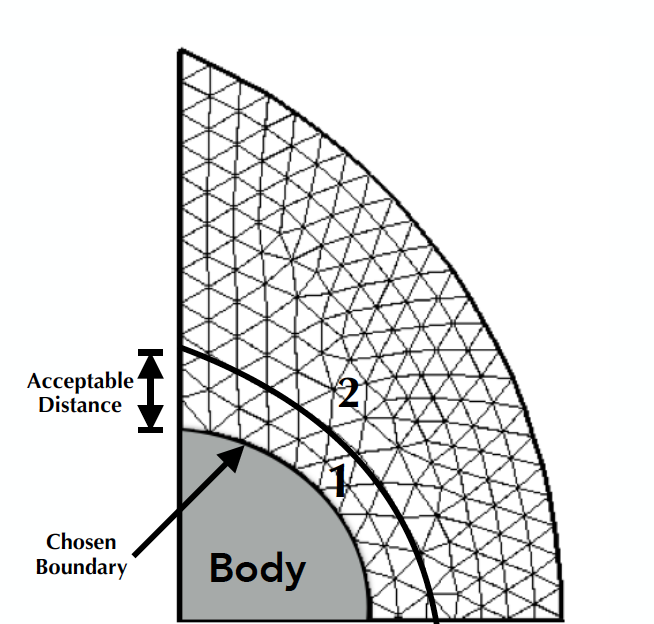
\includegraphics[scale=0.5]{Acce.png}}
\end{figure}
{\bf WATCH OUT:~} {\it If the option {\tt AcceptableDistance} is set on 0, this means that only one spring analogy will be applied to all the mesh}

\subsection{Mesh Fitting Parameters}
The mesh fitting techniques are defined as a post-process step.
\begin{lstlisting}[breaklines]
Simulator.SubSystem.DataPostProcessing          = DataProcessing
Simulator.SubSystem.DataPostProcessingNames     = MeFiAlgo
Simulator.SubSystem.MeFiAlgo.Comds              = MeshFittingAlgorithm
Simulator.SubSystem.MeFiAlgo.Data.CollaboratorNames = MeshAlgoLSS
\end{lstlisting}
The algorithm has a several characterizing parameters:\\
\newline
The Mesh adaptation is activated at a specific iteration.
\begin{lstlisting}[breaklines]
Simulator.SubSystem.MeFiAlgo.StartIter          = 0
Simulator.SubSystem.MeFiAlgo.SkipFirstIteration = true
\end{lstlisting}
The algorithm can be stopped by prescribing a maximum number of steps.
\begin{lstlisting}[breaklines]
Simulator.SubSystem.MeFiAlgo.StopIter           = 5000  
\end{lstlisting}
The option {\tt ProcessRate} will control the frequency of the use of the mesh refinement within the simulation.
\begin{lstlisting}[breaklines]
Simulator.SubSystem.MeFiAlgo.ProcessRate        = 20
\end{lstlisting}
The option {\tt updateVar} for the mesh fitting process needs to be consistent with the option {\tt updateVar} of the flow field computations (e.g. Rhoivt, cons)
\begin{lstlisting}[breaklines]
Simulator.SubSystem.MeFiAlgo.Names              = MeshFitting
Simulator.SubSystem.MeFiAlgo.Data.updateVar     = Cons
\end{lstlisting}
The linear springs are truncated and bounded between a minimum and maximum value based on a $P^2$ method, denoted respectively, minimum percentile and maximum percentile
\begin{lstlisting}[breaklines]
Simulator.SubSystem.MeFiAlgo.MeshFitting.minPercentile    = 0.30
Simulator.SubSystem.MeFiAlgo.MeshFitting.maxPercentile    = 0.55
\end{lstlisting}
An under-relaxation factor,  having a similar behavior as a mesh velocity, is added to the mesh adaptation solver to smooth the nodal displacements and avoid mesh node overlaps.
\begin{lstlisting}[breaklines]
Simulator.SubSystem.MeFiAlgo.MeshFitting.meshAcceleration = 0.05
\end{lstlisting}
{\bf WATCH OUT:~} {\it The {\tt meshAcceleration} option affects negatively the convergence rate. A trade-off between convergence issues in the flow field solver and convergence rate gives an order of magnitude of the under-relaxation factor of $\mathcal{O}(10^{-2})$}

The physics-driven adaptation, based on a physical flow field variable, is defined in the following options (e.g. density, pressure or temperature etc...) 
\begin{lstlisting}[breaklines]
Simulator.SubSystem.MeFiAlgo.MeshFitting.monitorVarID     = 4
Simulator.SubSystem.MeFiAlgo.MeshFitting.monitorPhysVarID = 0  
\end{lstlisting}
{\bf WATCH OUT:~} {\it If the {\tt monitorPhysVarID} is specified, it cancels the effect of the {\tt monitorVarID}}

The equilibrium spring length concerns the inner nodes and the multiplication factor {\tt ratioBoundaryToInnerEquilibriumSpringLength} tends to stiffen the boundary mesh nodes.
\begin{lstlisting}[breaklines]
Simulator.SubSystem.MeFiAlgo.MeshFitting.equilibriumSpringLength = 2e-4
Simulator.SubSystem.MeFiAlgo.MeshFitting.
                    ratioBoundaryToInnerEquilibriumSpringLength  = 0.01
\end{lstlisting}
The nodes on specific boundaries can be unlocked and therefore moving along a boundary line for 2D or a boundary surface for 3D.
\begin{lstlisting}[breaklines]
Simulator.SubSystem.MeFiAlgo.MeshFitting.unlockedBoundaryTRSs = SuperOutlet \
                                                                SlipWall
\end{lstlisting}
The last step will be to update the mesh 
\begin{lstlisting}[breaklines]
Simulator.SubSystem.CellCenterFVM.AfterMeshUpdateCom = StdMeshFittingUpdate
\end{lstlisting}
\subsection{Mesh Quality Indicator (MQI)}
A mesh quality indicator is a tool to qualitatively grade an adapted mesh.
One need to assign a specific value to the Mesh Quality Indicator depending on the mesh element type.\\
{\bf NOTE:~} {\it The Mesh Quality Indicator is mesh type dependant}
\begin{table}[H]
\centering
\label{my-label}
\begin{tabular}{cc}
\hline
Value & MQI                   \\
0     & deactivated option    \\
2     & 2D Triangular meshes  \\
3     & Aspect Ratio 2D Quads \\
4     & Skewness 2D Quads     \\
5     & 3D tetrahedral meshs  \\ \hline
\end{tabular}
\end{table}
\begin{lstlisting}[breaklines]
Simulator.SubSystem.MeFiAlgo.MeshFitting.MQIvalue = 0
\end{lstlisting}

\subsection{Refinement Stop Indicator (RSI)}
A Refinement Stop Indicator is a quantitative function aiming to stopping the refinement process at the best moment autonomously. It is based on user-defined tolerance on the mesh movement, expressed in percentage.\\
{\bf NOTE:~} {\it The  Refinement Stop Indicator is deactivated if the option {\tt tolerance = 0.}}
\begin{lstlisting}[breaklines]
Simulator.SubSystem.MeFiAlgo.MeshFitting.tolerance = 0.01
\end{lstlisting}

\subsection{Post-Processing - Outputs}
This section presents the different plottable outputs with \textbf{Tecplot} based on the predefined socket filled during the refinement process.\\
The option {\tt SocketNames} can be defined as following:
\begin{itemize}
\item {\tt stiffness }: For visualizing the mesh stiffness.
\item {\tt iradius   }: MQI for 2D triangular meshes
\item {\tt skewness  }: MQI for 2D quadrilateral meshes based on the skewness criteria 
\item {\tt AR        }: MQI for 2D quadrilateral meshes based on the aspect ratio criteria
\item {\tt isphere  }:  MQI for 3D tetrahedral meshes
\item {\tt relativeError }: For visualizing the value of the relative movement of the mesh nodes 
\end{itemize}

\begin{lstlisting}[breaklines]
Simulator.SubSystem.Tecplot.Data.DataHandleOutput.SocketNames   = stiffness
Simulator.SubSystem.Tecplot.Data.DataHandleOutput.VariableNames = kstiff
Simulator.SubSystem.Tecplot.Data.DataHandleOutput.isNodal = true
\end{lstlisting}

\begin{thebibliography}{00}
  
\bibitem{FParser} 
  J. Nieminen, J. Yliluoma. {\it Function Parser for C++},  http://warp.povusers.org/ FunctionParser/, 2009.

\bibitem{lani05} 
  A. Lani, T. Quintino, D. Kimpe, H. Deconinck, 
  {\it The COOLFluiD Framework - Design Solutions for High-Performance Object Oriented Scientific Computing Software}, 
  International Conference Computational Science 2005, Atlanta (GA), LNCS 3514, Vol.1, pp. 281-286, Springer-Verlag, 2005. 

\bibitem{lani06} 
  A. Lani, T. Quintino, D. Kimpe, H. Deconinck, S. Vandewalle and S. Poedts, 
  {\it Reusable Object-Oriented Solutions for Numerical Simulation of PDEs in a High Performance Environment}, 
  Scientific Programming. ISSN 1058-9244, Vol. 14, N. 2, pp. 111-139, IOS Press, 2006.

\bibitem{phd:lani}
  A. Lani, {\it An Object Oriented and High Performance Platform for Aerothermodynamics Simulation}, 
  Ph.D. thesis,von Karman Institute, Rhode-Saint-Gen\`ese, Belgium, 2008.
  
\bibitem{phd:magin}
  T. E. Magin, {\it A model for Inductive Plasma Wind Tunnels}, Ph.D. thesis, von Karman Institute, 
  Rhode-Saint-Gen\`ese, Belgium, 2004.

\bibitem{munafo10}
  A. Munafo, M. Panesi, R. Jaffe, A. Lani, T. Magin, 
  {\it Vibrational State to State Kinetics in Expanding and  Compressing Nitrogen Flows}, 
  AIAA-2010-4335, 10th AIAA/ASME Joint Thermophysics and Heat Transfer Conference, Chicago, Illinois, June 28-July 1, 2010. 
  
\bibitem{phd:panesi}
  M. Panesi, {\it Physical Models for Nonequilibrium Plasma Flow Simulations at High Speed Re-entry Conditions}, 
  Ph.D. thesis,von Karman Institute, Rhode-Saint-Gen\`ese, Belgium, 2009.

\bibitem{panesi09}
  M. Panesi, A. Lani and O. Chazot, {\it Reduced Kinetic Mechanism for CFD Applications}, 
  AIAA-2009-3920, 41st AIAA Thermophysics Conference, San Antonio, Texas, June 22-25, 2009.
  
\bibitem{phd:quintino}
  T. L. Quintino. {\it A Component Environment for High-Performance
    Scientific Computing. Design and Implementation},
  Ph.D. thesis,von Karman Institute, Rhode-Saint-Gen\`ese, Belgium, 2008.
  
\bibitem{phd:wuilbaut}
  Thomas Wuilbaut, {\it Algorithmic Developments for a Multiphysics Framework},  
  Ph.D. thesis,von Karman Institute, Rhode-Saint-Gen\`ese, Belgium, 2008.

\bibitem{dedner02}
  A. Dedner, F. Kemm, D. Kr\"oner, C. D. Munz, T. Schnitzer and M. Wesenberg,
  {\it Hyperbolic Divergence Cleaning for the MHD Equations},
  Journal of Computational Physics, Vol. 175, pp. 645-673, 2002, doi:10.1006/jcph.2001.6961.

\bibitem{powell95}
  K. G. Powell, P. L. Roe, R. S. Myong, T. I. Gombosi and D. L. De Zeeuw,
  {\it An Upwind Scheme for Magnetohydrodynamics},
  $12^{th}$ AIAA Computational Fluid Dynamics Conference, p. 661-674, Am. Inst. of Aeron. and Astron., San Diego, Calif., 1995.

\bibitem{powell99}
  K. G. Powell, P. L. Roe, T. J. Linde, T. I. Gombosi and D. L. De Zeeuw,
  {\it A Solution-Adaptive Upwind Scheme for Ideal Magnetohydrodynamics},
  Journal of Computational Physics, Vol. 154, pp. 284-309, 1999, doi:10.1006/jcph.1999.6299.

\bibitem{tanaka94}
  T. Tanaka, {\it Finite Volume TVD Scheme on an Unstructured Grid System for Three-Dimensional MHD Simulation of Inhomogeneous Systems Including Strong Background Potential Fields},
  Journal of Computational Physics, Vol. 111, pp. 381-389, 1994, doi:10.1006/jcph.1994.1071.

\bibitem{yalim08}
  M. S. Yalim, D. Vanden Abeele and A. Lani, 
  {\it Simulation of Field-aligned Ideal MHD Flows around Perfectly Conducting Cylinders Using an Artificial Compressibility Approach}, 
  Proceedings of the $11^{th}$ International Conference on Hyperbolic Problems held in Ecole Normale Sup\'erieure, Lyon, France, July 17-21, 2006, pp. 1085-1092, Springer-Verlag, 2008.

\bibitem{phd:yalim}
  M. S. Yalim, {\it An Artificial Compressibility Analogy Approach for Compressible Ideal MHD: Application to Space Weather Simulation},
  Ph.D. thesis,von Karman Institute, Rhode-Saint-Gen\`ese, Belgium, 2008.

\bibitem{yalim11jcp}
  M. S. Yalim, D. Vanden Abeele, A. Lani, T. Quintino and H. Deconinck,
  {\it A Finite Volume Implicit Time Integration Method for Solving the Equations of Ideal Magnetohydrodynamics for the Hyperbolic Divergence Cleaning Approach},
  Journal of Computational Physics, Vol. 230, N. 15, pp. 6136-6154, 2011, doi:10.1016/j.jcp.2011.04.020.

\bibitem{yalim11jgr}
  M. S. Yalim, J. Majewski, H. Deconinck and S. Poedts,
  {\it Adaptive Unstructured Grid Simulation of Interaction of Solar Wind with Planetary Magnetosphere Using an Implicit Finite Volume Method},
  Journal of Geophysical Research Space Physics, submitted, 2011.
  
\end{thebibliography}

\end{document}
